\section* {1.1. Решение СЛАУ с помощью LU-разложения матриц}


\subsection{Постановка задачи}
Реализовать алгоритм LU -  разложения матриц (с выбором главного элемента) в виде программы. Используя разработанное программное обеспечение, решить систему линейных алгебраических уравнений (СЛАУ). Для матрицы СЛАУ вычислить определитель и обратную матрицу. 

{\bfseries Вариант:} 5
\begin{align*}
& \begin{cases}
3x_1 - 8x_2 + x_3 - 7x_4 = 96,\\
6x_1 + 4x_2 + 8x_3 + 5x_4 = -13,\\
-x_1 + x_2 - 9x_3 - 3x_4 = -54,\\
-6x_1 + 6x_2 + 9x_3 - 4x_4 = 82.
\end{cases} \\
\end{align*}

\subsection{Результаты работы}
\begin{figure}[h!]
\raggedright
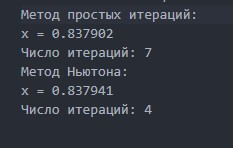
\includegraphics[width=.8\textwidth]{img1}
\end{figure}
\pagebreak

\subsection{Исходный код}
\lstinputlisting{include/1.cpp}
\pagebreak

\section* {1.2. Решение СЛАУ методом прогонки}

\setcounter{subsection}{0}

\subsection{Постановка задачи}
Реализовать метод прогонки в виде программы, задавая в качестве входных данных ненулевые элементы матрицы системы и вектор правых частей. Используя разработанное программное обеспечение, решить СЛАУ с трехдиагональной матрицей.    

{\bfseries Вариант:} 5
\begin{align*}
& \begin{cases}
8x_1 + 4x_2 = 48,\\
-5x_1 + 22x_2 + 8x_3 = 125,\\
-5x_2 - 11x_3 + x_4 = -43,\\
-9x_3 - 15x_4 + x_5 = 18, \\
x_4 + 7x_5 = -23.
\end{cases} \\
\end{align*}

\subsection{Результаты работы}
\begin{figure}[h!]
\raggedright
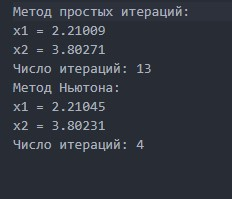
\includegraphics[width=.8\textwidth]{img2}
\end{figure}
\pagebreak

\subsection{Исходный код}
\lstinputlisting{include/2.cpp}
\pagebreak

\section* {1.3. Решение СЛАУ методом простых итераций и методом Зейделя}

\setcounter{subsection}{0}

\subsection{Постановка задачи}
Реализовать метод простых итераций и метод Зейделя в виде программ, задавая в качестве входных данных матрицу системы, вектор правых частей и точность вычислений. Используя разработанное программное обеспечение, решить СЛАУ. Проанализировать количество итераций, необходимое для достижения заданной точности.    

{\bfseries Вариант:} 5
\begin{align*}
& \begin{cases}
20x_1 + 5x_2 + 7x_3 + x_4 = -117,\\
-x_1 + 13x_2 - 7x_4 = -1,\\
4x_1 - 6x_2 + 17x_3 + 5x_4 = 49,\\
-9x_1 + 8x_2 + 4x_3 - 25x_4 = -21, \\
x_4 + 7x_5 = -23.
\end{cases} \\
\end{align*}

\subsection{Результаты работы}
\begin{figure}[h!]
\raggedright
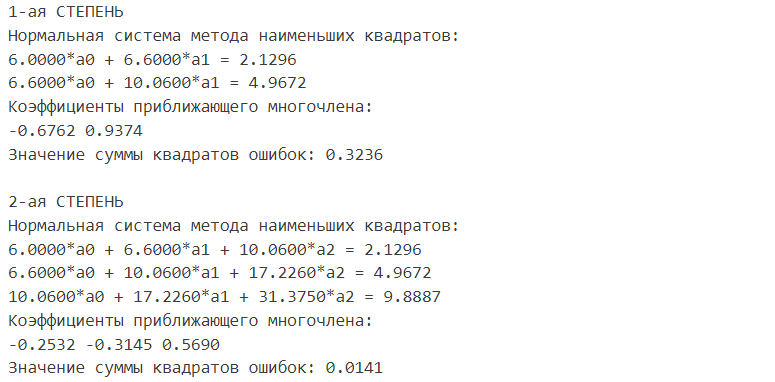
\includegraphics[width=.9\textwidth]{img3}
\end{figure}
\pagebreak

\subsection{Исходный код}
\lstinputlisting{include/3.cpp}
\pagebreak

\section* {1.4. Нахождение СЗ и СВ симметрических матриц методом вращений}

\setcounter{subsection}{0}

\subsection{Постановка задачи}
Реализовать метод вращений в виде программы, задавая в качестве входных данных матрицу и точность вычислений. Используя разработанное программное обеспечение, найти собственные значения и собственные векторы симметрических матриц. Проанализировать зависимость погрешности вычислений от числа итераций.    

{\bfseries Вариант:} 5
\begin{align*}
& \begin{pmatrix}
0 & -7 & 7 \\
-7 & -9 & -5 \\
7 & -5 & -1
\end{pmatrix} \\
\end{align*}

\subsection{Результаты работы}
\begin{figure}[h!]
\raggedright
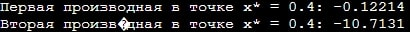
\includegraphics[width=1.1\textwidth]{img4}
\end{figure}
\pagebreak

\subsection{Исходный код}
\lstinputlisting{include/4.cpp}
\pagebreak

\section* {1.5. Нахождение СЗ и СВ матриц алгоритмом QR-разложения}

\setcounter{subsection}{0}

\subsection{Постановка задачи}
Реализовать алгоритм QR – разложения матриц в виде программы. На его основе разработать программу, реализующую QR – алгоритм решения полной проблемы собственных значений произвольных матриц, задавая в качестве входных данных матрицу и точность вычислений. С использованием разработанного программного обеспечения найти собственные значения матрицы.    

{\bfseries Вариант:} 5
\begin{align*}
& \begin{pmatrix}
5 & 8 & -2 \\
7 & -2 & -4 \\
5 & 8 & -1
\end{pmatrix} \\
\end{align*}

\subsection{Результаты работы}
\begin{figure}[h!]
\raggedright
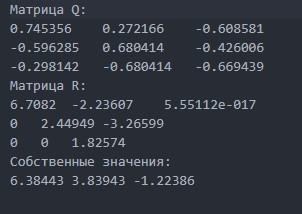
\includegraphics[width=1.1\textwidth]{img5}
\end{figure}
\pagebreak

\subsection{Исходный код}
\lstinputlisting{include/5.cpp}
\pagebreak